% Options for packages loaded elsewhere
% Options for packages loaded elsewhere
\PassOptionsToPackage{unicode}{hyperref}
\PassOptionsToPackage{hyphens}{url}
\PassOptionsToPackage{dvipsnames,svgnames,x11names}{xcolor}
%
\documentclass[
  sn-basic,
  10pt,
]{sn-jnl}


\usepackage{xcolor}
\usepackage{amsmath,amssymb}
\setcounter{secnumdepth}{5}
\usepackage{iftex}
\ifPDFTeX
  \usepackage[T1]{fontenc}
  \usepackage[utf8]{inputenc}
  \usepackage{textcomp} % provide euro and other symbols
\else % if luatex or xetex
  \usepackage{unicode-math} % this also loads fontspec
  \defaultfontfeatures{Scale=MatchLowercase}
  \defaultfontfeatures[\rmfamily]{Ligatures=TeX,Scale=1}
\fi
\usepackage{lmodern}
\ifPDFTeX\else
  % xetex/luatex font selection
\fi
% Use upquote if available, for straight quotes in verbatim environments
\IfFileExists{upquote.sty}{\usepackage{upquote}}{}
\IfFileExists{microtype.sty}{% use microtype if available
  \usepackage[]{microtype}
  \UseMicrotypeSet[protrusion]{basicmath} % disable protrusion for tt fonts
}{}
% Make \paragraph and \subparagraph free-standing
\makeatletter
\ifx\paragraph\undefined\else
  \let\oldparagraph\paragraph
  \renewcommand{\paragraph}{
    \@ifstar
      \xxxParagraphStar
      \xxxParagraphNoStar
  }
  \newcommand{\xxxParagraphStar}[1]{\oldparagraph*{#1}\mbox{}}
  \newcommand{\xxxParagraphNoStar}[1]{\oldparagraph{#1}\mbox{}}
\fi
\ifx\subparagraph\undefined\else
  \let\oldsubparagraph\subparagraph
  \renewcommand{\subparagraph}{
    \@ifstar
      \xxxSubParagraphStar
      \xxxSubParagraphNoStar
  }
  \newcommand{\xxxSubParagraphStar}[1]{\oldsubparagraph*{#1}\mbox{}}
  \newcommand{\xxxSubParagraphNoStar}[1]{\oldsubparagraph{#1}\mbox{}}
\fi
\makeatother


\usepackage{longtable,booktabs,array}
\usepackage{calc} % for calculating minipage widths
% Correct order of tables after \paragraph or \subparagraph
\usepackage{etoolbox}
\makeatletter
\patchcmd\longtable{\par}{\if@noskipsec\mbox{}\fi\par}{}{}
\makeatother
% Allow footnotes in longtable head/foot
\IfFileExists{footnotehyper.sty}{\usepackage{footnotehyper}}{\usepackage{footnote}}
\makesavenoteenv{longtable}
\usepackage{graphicx}
\makeatletter
\newsavebox\pandoc@box
\newcommand*\pandocbounded[1]{% scales image to fit in text height/width
  \sbox\pandoc@box{#1}%
  \Gscale@div\@tempa{\textheight}{\dimexpr\ht\pandoc@box+\dp\pandoc@box\relax}%
  \Gscale@div\@tempb{\linewidth}{\wd\pandoc@box}%
  \ifdim\@tempb\p@<\@tempa\p@\let\@tempa\@tempb\fi% select the smaller of both
  \ifdim\@tempa\p@<\p@\scalebox{\@tempa}{\usebox\pandoc@box}%
  \else\usebox{\pandoc@box}%
  \fi%
}
% Set default figure placement to htbp
\def\fps@figure{htbp}
\makeatother





\setlength{\emergencystretch}{3em} % prevent overfull lines

\providecommand{\tightlist}{%
  \setlength{\itemsep}{0pt}\setlength{\parskip}{0pt}}





%%%% Standard Packages

\usepackage{graphicx}%
\usepackage{multirow}%
\usepackage{amsmath,amssymb,amsfonts}%
\usepackage{amsthm}%
\usepackage{mathrsfs}%
\usepackage[title]{appendix}%
\usepackage{xcolor}%
\usepackage{textcomp}%
\usepackage{manyfoot}%
\usepackage{booktabs}%
\usepackage{algorithm}%
\usepackage{algorithmicx}%
\usepackage{algpseudocode}%
\usepackage{listings}%
\usepackage{setspace}%
\usepackage{mathtools}%




%%%%

\raggedbottom
\makeatletter
\@ifpackageloaded{caption}{}{\usepackage{caption}}
\AtBeginDocument{%
\ifdefined\contentsname
  \renewcommand*\contentsname{Table of contents}
\else
  \newcommand\contentsname{Table of contents}
\fi
\ifdefined\listfigurename
  \renewcommand*\listfigurename{List of Figures}
\else
  \newcommand\listfigurename{List of Figures}
\fi
\ifdefined\listtablename
  \renewcommand*\listtablename{List of Tables}
\else
  \newcommand\listtablename{List of Tables}
\fi
\ifdefined\figurename
  \renewcommand*\figurename{\textbf{Fig.}}
\else
  \newcommand\figurename{\textbf{Fig.}}
\fi
\ifdefined\tablename
  \renewcommand*\tablename{Table}
\else
  \newcommand\tablename{Table}
\fi
}
\@ifpackageloaded{float}{}{\usepackage{float}}
\floatstyle{ruled}
\@ifundefined{c@chapter}{\newfloat{codelisting}{h}{lop}}{\newfloat{codelisting}{h}{lop}[chapter]}
\floatname{codelisting}{Listing}
\newcommand*\listoflistings{\listof{codelisting}{List of Listings}}
\usepackage{amsthm}
\theoremstyle{plain}
\newtheorem{corollary}{Corollary}[section]
\theoremstyle{plain}
\newtheorem{proposition}{Proposition}[section]
\theoremstyle{remark}
\AtBeginDocument{\renewcommand*{\proofname}{Proof}}
\newtheorem*{remark}{Remark}
\newtheorem*{solution}{Solution}
\newtheorem{refremark}{Remark}[section]
\newtheorem{refsolution}{Solution}[section]
\makeatother
\makeatletter
\makeatother
\makeatletter
\@ifpackageloaded{caption}{}{\usepackage{caption}}
\@ifpackageloaded{subcaption}{}{\usepackage{subcaption}}
\makeatother
\usepackage{bookmark}
\IfFileExists{xurl.sty}{\usepackage{xurl}}{} % add URL line breaks if available
\urlstyle{same}
\hypersetup{
  pdftitle={Learning growth mechanisms of tail realistic preferential attachment models from network degree distributions},
  pdfauthor={Thomas William Boughen; Clement Lee; Vianey Palacios Ramirez},
  pdfkeywords={Network degrees · Discrete extremes · Power law ·
Preferential attachment},
  colorlinks=true,
  linkcolor={blue},
  filecolor={Maroon},
  citecolor={Blue},
  urlcolor={Blue},
  pdfcreator={LaTeX via pandoc}}




\title[Learning growth mechanisms of tail realistic preferential
attachment models from network degree distributions]{Learning growth
mechanisms of tail realistic preferential attachment models from network
degree distributions}

% author setup
\author*[1]{\fnm{Thomas William} \sur{Boughen}}\email{t.w.boughen1@newcastle.ac.uk}\author[1]{\fnm{Clement} \sur{Lee}}\author[1]{\fnm{Vianey Palacios} \sur{Ramirez}}
% affil setup
\affil[1]{\orgdiv{School of Mathematics, Statistics and
Physics}, \orgname{Newcastle University}}

% abstract 
\abstract{Identifying the generating mechanism of a network is
challenging as, more often than not, only snapshots are available, but
not the full evolution. One candidate for the generating mechanism is
preferential attachment which, in its simplest form, results in a degree
distribution that follows the power law. Consequently, the growth of
real-life networks that display such power-law behaviour is commonly
modelled by preferential attachment. The ubiquity of the power law has
been challenged by the presence of alternatives with comparable
performance, as well as the recent findings that the tail of the degree
distribution is often lighter than implied by the body, whilst still
being regularly varying. In this paper, we propose a preferential
attachment model with a flexible preference function. Using methods for
discrete extremes, we characterise the tail behaviour of the limiting
degree distribution directly by the form of the preference function.
Directly relating the tail index to the model parameters enables them to
be inferred when fitting to degree distributions alone, which is
supported by simulation studies. Results of applications to real data
are promising and comparable to alternatives.}

% keywords
\keywords{Network degrees · Discrete extremes · Power law · Preferential
attachment}


\pacs[\sffamily AMS 2000 Subject Classification]{05C80· 60J85· 62G32}

\begin{document}
\maketitle


\newpage

\section{Introduction}\label{introduction}

Networks have become powerful tools for representing and analysing
complex systems, with uses in a large array of fields. In network
science and statistics, they have been studied by various families of
models, from stochastic block models for detecting communities online
\citep{Latouche11}, to exponential random graph models (ERGMs) for
analysing the global trade network \citep{Setayesh22}, and mechanistic
models for investigating patterns in neural systems \citep{Betzel17}.

Amid the recent rise of interest in networks, there has been a debate on
whether most real networks are scale-free. Claiming a real network is
scale-free is equivalent to saying that the tail of the degree
distribution follows a power law, that is the fraction of nodes with
degree greater than \(k\) is eventually proportional to \(k^{-\alpha}\),
and therefore has a regularly varying tail with tail index \(\alpha\).
On the side against the claim, that most real networks are scale-free,
is \citet{Broido_2019} who compared the fits of a power law model
against that of several non-scale-free models to nearly a thousand
networks, only to find strong evidence for scale-freeness in four
percent and weak evidence in over half of the networks, thus claiming
that scale-free networks do not make up a majority of real networks.
\citet{Voitalov_2019} disagree and claim that these networks are not
nearly as rare and only appear so as a result of an unrealistic
expectation of a power law without deviations or noise. Additional
evidence of these deviations from a power law is shown by \citet{Lee24}
who demonstrate that a lot of networks are partially scale-free, in that
the body of the degree distribution is often modelled well by a power
law, while the tail is lighter than what is implied by the body, albeit
still regularly varying.

The popularity of using the power law for network degrees can be traced back to a preferential attachment (PA) model popularised by \cite{Barabasi99}. In the general model, general preferential attachment (GPA), as new nodes join the network, an existing node with degree $k$ gains edges at a rate proportional to $b(k)$, where $b(\cdot)$ is a non-negative preference function. \cite{Barabasi99} showed that, when $b(k) = k + 1$, in the limit the resulting degree distribution is regularly varying with index 2 --- this model is commonly known as the Barab\'asi-Albert (BA) model.  Subsequently, if a real network is shown to be scale-free, one can loosely justify PA as the underlying mechanism of its growth.

Nevertheless, most studies into the appropriateness of a power law for
the degrees of real networks, the aforementioned references included,
have been largely descriptive in the sense that no information about the
growth of the networks is revealed.

The model from \citet{Barabasi99} provided the foundations for various
generalisations --- \citet{krapivsky01} considered
\(b(k) = (k+1)^\alpha\), and showed that the tail of the degree
distribution is not regularly varying (and therefore not following the
power law) when \(0<\alpha<1\), and when \(\alpha>1\) a finite number of
nodes end up with all edges after a certain point resulting in a
degenerate degree distribution. \citet{wang2022random} return to a
linear preference function of the form \(b(k) = k+\varepsilon\) but add
the possibility for reciprocal edges to be sent, resulting in the joint
distribution of in-degree and out-degree being multivariate regularly
varying and having the property of hidden regular variation.
\citet{rudas07} followed in the footsteps of \citet{krapivsky01}, by
considering a GPA tree and using theory from continuous branching
processes, deriving a limiting degree distribution in terms of the
preference function \(b(\cdot)\). Unfortunately, research in this area
tends to only focus on the theoretical asymptotic results of network
growth models with little analysis of real networks.

This paper aims to address the gap between the applied and theoretical
works, by asking if a network is assumed to come from a GPA model, can
we use the degree distribution alone to directly infer the parameters of
the the preference function and learn about the growth mechanisms?
Moreover, proper consideration is given to the tail of the degree
distribution, because otherwise the effects of the largest degrees,
which correspond to the most influential nodes, deviating from the power
law will be discounted.

\citet{Voitalov_2019} have pioneered using methods in extreme value
theory to analyse degree distributions and while their approach is good
they overlooked the inapplicability of standard tools for continuous
extremes, due to the discrete nature of degrees. A key difficulty arises
because many standard discrete distributions, such as the Poisson,
geometric, or negative binomial, do not satisfy the conditions required
to belong to a maximum domain of attraction (MDA). \citet{shimura12}
showed that a discrete distribution \(F\) must be long-tailed, that is
\(\lim_{x\rightarrow\infty}\bar F(x+1)/\bar F(x) = 1\), in order to be
in an MDA, and introduced the notion of recoverability to the MDA, also
sometimes referred to as the discrete MDA \citep{hitz24}. Using the
theoretical guarantees of being in a discrete MDA for a discrete
distribution by \citet{shimura12}, we demonstrate how the tail of the
degree distribution is directly influenced by \(b(\cdot)\), and
subsequently propose a class of preference functions that not only imply
regularly varying degree distributions but are also tail realistic for
real networks. These analytical results enable the likelihood of the
degree distribution to be expressed in terms of the parameters of
\(b(\cdot)\), which in turn allows the underlying mechanism of the
network, assumed to grow according to GPA, to be inferred directly.

The remainder of the paper is as follows: Section~\ref{sec-tail} gives a
detailed description of the GPA model alongside the theoretical results
for the survival function of the limiting degree distribution, with a
focus on the tail behaviour in terms of the preference function
\(b(\cdot)\). A class of asymptotically linear preference functions will
be introduced and shown to guarantee regular variation in the degree
distribution while remaining flexible up until a threshold.
Section~\ref{sec-model} utilises the proposed preference function and
illustrates numerically how the tail index of the degree distribution
varies with the model parameters. The simulation study in
Section~\ref{sec-sim} demonstrates that the parameters can be recovered
from fitting the model to only the degree distribution and as a
consequence recover the underlying growth mechanism.
Section~\ref{sec-real} fits the model to some real data and provides
posterior estimates for the preference function. Section~\ref{sec-conc}
provides a discussion of this paper and possible avenues for future
work.

\section{Tail Behaviour of GPA Model}\label{sec-tail}

The model that we will focus on in this paper is the General
Preferential Attachment (GPA) model in \citet{rudas07} and is defined as
follows:

Starting at time \(t=0\) with an initial network of \(m\) vertices that
each have no edges, at times \(t=1,2,\ldots\) a new vertex is added to
the network bringing with it \(m\) directed edges from the new vertex;
the targets for each of these edges are selected from the vertices
already in the network with weights proportional to some non-decreasing
preference function \(b(\cdot)\) of their degree, where
\(b: \mathbb N \mapsto \mathbb R^+\setminus\{0\}\) is such that:

\begin{equation}\phantomsection\label{eq-condb2}{
\sum_{k=0}^\infty\frac{1}{b(k)} = \infty.
}\end{equation}

Special cases of this model include the BA model when $b(k) = k+1$, which in the limit of $t\rightarrow \infty$ leads to a power-law degree distribution with tail index 2, and the Uniform Attachment (UA) model where $b(k)=c$ leading to a degree distribution with a tail that is not regularly varying.

The survival function of the limiting degree distribution, called the
limiting survival hereafter, under condition \ref{eq-condb2} can be
analytically derived in the case where \(m=1\), which is presented
below.

Consider a continuous time branching process \(\zeta(t)\) driven by a
Markovian pure birth process, with \(\zeta(0)=0\) and birth rates
depending on a non-negative function \(b(\cdot)\): \[
\Pr(\zeta(t+\text{d}t)=k+1|\zeta(t)=k) = b(k)\text{d}t + o(\text{d}t).
\] Denote the density of the point process associated with the pure
birth process corresponding to the growth of an individual node by
\(\rho(t)\), and its Laplace transform by
\(\hat \rho(\lambda)\coloneqq \int_0^\infty e^{-\lambda t}\rho(t)\text{d}t\).
We denote the Malthusian parameter of this process by \(\lambda^*\),
that is \(\lambda^*\) satisfies \(\hat\rho(\lambda^*) = 1\).

Now, we construct the tree \(\Upsilon(t)\) determined by \(\zeta(t)\) as
follows: \(\Upsilon(0)=\{\emptyset\}\) and \(\Upsilon(t)\) is a graph
where each existing node \(x\) in \(\Upsilon(t)\) gives birth to a child
with rate \(b(\mathrm{deg}(x, \Upsilon(t)))\) independently of the other
nodes where \(\mathrm{deg}(x, \Upsilon(t))\) is the degree of node \(x\)
in the tree \(\Upsilon(t)\) at time \(t\), denote by
\(\Upsilon(t)_{\downarrow x}\) the tree when treating node \(x\) as the
root.

The limiting survival can be viewed as the limit over time of the
empirical proportion of vertices with degree over a threshold
\(k\in\mathbb N\), that is:

\[
\bar F(k) = \lim_{t\rightarrow\infty}\frac{\sum_{x\in\Upsilon(t)}\mathbb I\left\{\text{deg}(x,\Upsilon(t)_{\downarrow x})>k\right\}}{\sum_{x\in\Upsilon(t)} 1},
\] for the tree \(\Upsilon(t)\) defined as above, Theorem 1 from
\citet{rudas07} states that

\begin{equation}\phantomsection\label{eq-survlim}{
\lim_{t\rightarrow\infty}\frac{1}{|\Upsilon(t)|}\sum_{x\in\Upsilon(t)}\varphi(\Upsilon(t)_{\downarrow x}) = \lambda^* \int_0^\infty e^{-\lambda^* t}\mathbb E\left[\varphi(\Upsilon(t))\right]\text{d}t.
}\end{equation}

Using this result, and the characteristic function
\(\varphi(\Upsilon(t)_{\downarrow x}) = \mathbb I\{\text{deg}(x,\Upsilon(t)_{\downarrow x})>k\}\),
we can write the limiting survival as:

\begin{equation}\phantomsection\label{eq-surv-origin}{
\bar F(k) = \frac{\int_0^\infty e^{-\lambda^* t}\mathbb E\left[\mathbb I\left\{\text{deg}(x,\Upsilon(t))>k\right\}\right]\text{d}t}{\int_0^\infty e^{-\lambda^* t}\text{d}t} = \prod_{i=0}^k\frac{b(i)}{\lambda^* + b(i)}.
}\end{equation}

Therefore, the corresponding probability mass function of the degree
distribution \(f(k) = \bar F(k-1) - \bar F(k)\) is

\begin{equation}\phantomsection\label{eq-pmf-origin}{
f(k) = \frac{\lambda^*}{\lambda^* + b(k)}\prod_{i=0}^{k-1}\frac{b(i)}{\lambda^*+b(i)}.
}\end{equation}

We now investigate how the tail behaviour of the discrete limiting
degree distribution is influenced by the preference function \(b(·)\),
using the characterisation by \citet{shimura12}.

A central tool of this characterisation is the quantity \(\Omega(F,k)\).
For a discrete distribution \(F\) with survival function \(\bar F\) and
\(k\in\mathbb Z^+\) define:

\[
\Omega(F,k) = \left(\log\displaystyle\frac{\bar F (k+1)}{\bar F (k+2)}\right)^{-1} - \left(\log\displaystyle\frac{\bar F (k)}{\bar F (k+1)}\right)^{-1}.
\]

@shimura12 established that if $\lim_{k\rightarrow\infty} \Omega(F,k) = 1/\alpha$ ($\alpha>0$), then $F$ is regularly varying with $\bar F(k) \sim k^{-\alpha}$, and hence belongs to the Fr\'echet MDA with tail index $\alpha$. If instead, $\lim_{k\rightarrow\infty} \Omega(F,k) = 0$ then the distribution is recoverable to the Gumbel MDA; in this cases we say that the distribution is light-tailed. Moreover, if the distribution is also long-tailed, we can conclude that $F$ itself lies in the Gumbel MDA.

This framework offers a natural approach for analysing the tail
behaviour of the limiting degree distribution. The following proposition
gives the limiting behaviour of \(\Omega(F,k)\) when \(F\) is a limiting
degree distribution resulting from the GPA model with preference
function \(b(\cdot)\).

\begin{proposition}[]\protect\hypertarget{prp-omega}{}\label{prp-omega}

Let \(\bar F (k)\) be the limiting survival function of degrees in a GPA
network with preference function \(b\) such that
\(b(k)\rightarrow\infty\). Then: \[
\lim_{k\rightarrow\infty}\Omega(F,k) = \lim_{k\rightarrow\infty}\frac{b(k+1)-b(k)}{\lambda^*}.
\]

Here, \(\lambda^*\) is the Malthusian parameter of the corresponding
branching process. See Appendix \ref{sec-prpproof} for the details of
the proof.

\end{proposition}

\begin{refremark}
If \(\lim_{k\rightarrow\infty}b(k)<\infty\), then \(\Omega(F, k) = 0\).
Furthermore, \(F\) is recovered to the Gumbel MDA but does not belong to
the Gumbel MDA itself as it is not long-tailed. See Appendix
\ref{sec-remproof} for the proof.

\label{rem-omega}

\end{refremark}

\begin{corollary}[]\protect\hypertarget{cor-omega2}{}\label{cor-omega2}

Let \(\bar F (k)\) be the limiting survival function of degrees in a GPA
network with preference function \(b\) such that
\(b(k)\rightarrow\infty\). Then:

\begin{itemize}
\item
  \(\bar F(k)\) is regularly varying if and only if
  \(\lim_{k\rightarrow\infty}[b(k+1)-b(k)]=c>0\), in which case the tail
  index is \(\lambda^*/c\), where \(\lambda^*\) is the Malthusian
  parameter of the corresponding branching process.
\item
  \(\bar F(k)\) is light-tailed if and only if
  \(\lim_{k\rightarrow\infty}[b(k+1)-b(k)]=0\). Further, \(F\) is in the
  Gumbel MDA as it is also long-tailed.
\end{itemize}

\end{corollary}

Corollary~\ref{cor-omega2} is a direct consequence of
Proposition~\ref{prp-omega} and the results of \citet{shimura12}, and it
aligns with previous findings in the literature. In particular it is
consistent with \citet{krapivsky01}, who showed that a sub-linear
preference function leads to a light-tailed distributions, since for
\(b(k)=k^\alpha\) with \(\alpha<1\), we have
\(\lim_{k\rightarrow\infty}[b(k+1)-b(k)]=0\). Conversely, it also agrees
with the limiting behaviour of the BA model, which produces a regularly
degree distribution with tail index 2; for the preference function
\(b(k)=k+1\), \(\lim_{k\rightarrow\infty}[b(k+1)-b(k)]=1\), giving a
tail index of \(\lambda^*=2\). We can also obtain the afforementioned
results for UA, taking \(b(k)=c\) it is clear that
\(\lim_{k\rightarrow\infty}b(k)<\infty\) and therefore by
Remark~\ref{rem-omega} we have tha
\(\lim_{k\rightarrow\infty}\Omega(F,k)=0\) meaning \(F\)'s tail is not
regularly varying and is in the Gumbel domain as \(b(k)\) is also
long-tailed.

Using Corollary~\ref{cor-omega2} we can directly connect the preference
function to the tail behaviour of the degree distribution. By choosing
an appropriate preference function, we can ensure that the tail of the
degree distribution is regularly varying while allowing the body to
deviate from the power-law shape, as observed in real networks. Inspired
by \citet{Lee24}, we consider a piecewise function:

\begin{equation}\phantomsection\label{eq-pref}{
b(k) = \begin{cases}
k^\alpha + \varepsilon,&k\le k_0,\\
k_0^\alpha + \varepsilon + \beta(k-k_0), &k> k_0
\end{cases}
}\end{equation} for \(\alpha,\beta, \varepsilon>0\) and
\(k_0\in\mathbb N\). By Corollary~\ref{cor-omega2}, the resulting degree
distribution is regularly varying with tail index \(\lambda^*/\beta\),
since
\(\lim_{k\rightarrow\infty}\Omega(F,k) = \frac{\beta}{\lambda^*}\).

Shown in Figure~\ref{fig-ex} is an example of one such preference
function of this form, the value of \(\varepsilon\) controls the
baseline appeal of a node with zero degree and \(k_0\) controls the
point at which the behaviour changes, below this point the curvature of
the function is controlled by the value of \(\alpha\) and above \(k_0\)
the gradient of the linear section is contolled by \(\beta\).

\begin{figure}

\centering{

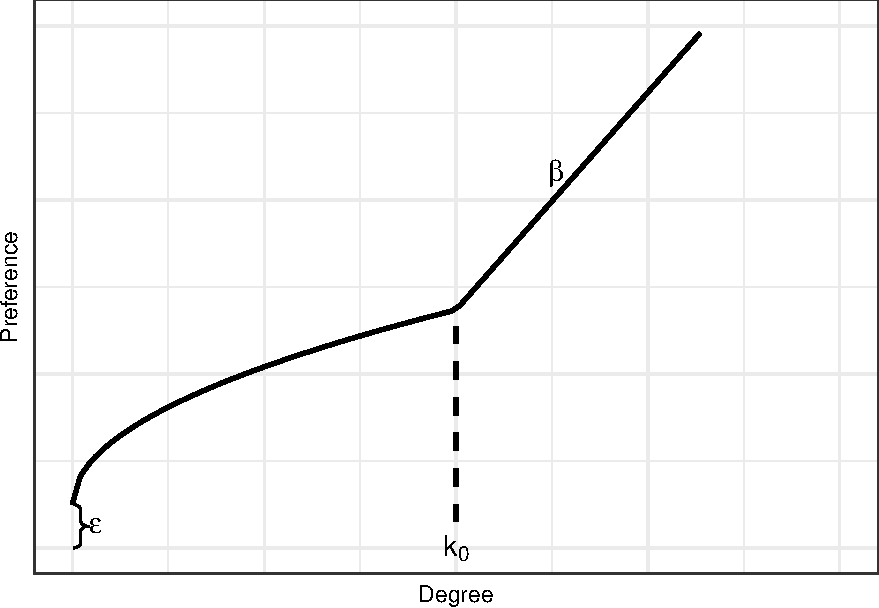
\includegraphics[width=119mm,height=\textheight,keepaspectratio]{paper_files/figure-pdf/fig-ex-1.pdf}

}

\caption{\label{fig-ex}Example construction of the preference function
in Equation~\ref{eq-pref}}

\end{figure}%

\newpage

\section{A Tail-realistic GPA model}\label{sec-model}

In the previous section, we constructed an asymptotically linear
preference function that allows for the inclusion of sub/super-linear
behaviour below the threshold, while simultaneously guaranteeing regular
variation of the degrees. In this section, we demonstrate the
flexibility of the proposed GPA model, that is using the preference
function from Equation~\ref{eq-pref} in the GPA model, with regard to
the tail behaviour of the limiting degree distribution. The limiting
survival of the proposed GPA model is:

\begin{equation}\phantomsection\label{eq-polysurv}{
\bar F(k) = \begin{cases}
\prod_{i=0}^{k}\frac{i^\alpha + \varepsilon}{\lambda^*+i^\alpha + \varepsilon},&k\le k_0,\\
\left(\prod_{i=0}^{k_0-1}\frac{i^\alpha + \varepsilon}{\lambda^*+i^\alpha + \varepsilon}\right)\frac{\Gamma(\lambda^*+k_0^\alpha + \varepsilon)/\beta)}{\Gamma\left((k_0^\alpha + \varepsilon)/\beta\right)} \frac{\Gamma\left(k-k_0 + 1 +\frac{k_0^\alpha + \varepsilon}{\beta}\right)}{\Gamma\left(k-k_0 + 1 +\frac{\lambda^* +k_0^\alpha + \varepsilon}{\beta}\right)},&k > k_0,
\end{cases}
}\end{equation} with Malthusian parameter \(\lambda^*\) satisfying
\(\hat \rho(\lambda^*)=1\) where

\begin{equation}\phantomsection\label{eq-rho}{
\hat\rho(\lambda) = \sum_{n=0}^{k_0}\prod_{i=0}^{n-1}\frac{i^\alpha + \varepsilon}{\lambda+i^\alpha + \varepsilon} + \left(\frac{k_0^\alpha + \varepsilon}{\lambda-\beta}\right)\prod_{i=0}^{k_0-1}\frac{i^\alpha + \varepsilon}{\lambda + i^\alpha + \varepsilon}, 
}\end{equation} which has to be solved numerically for most parameter
choices. Also, note that \(\lambda>\beta\). See Appendix
\ref{sec-rhoproof} for the derivations of Equation~\ref{eq-rho}.

For some parameter combinations, the limiting survival \(\bar F(k)\) is
shown on log-log scale in Figure~\ref{fig-polylinsurv}:

\begin{figure}

\centering{

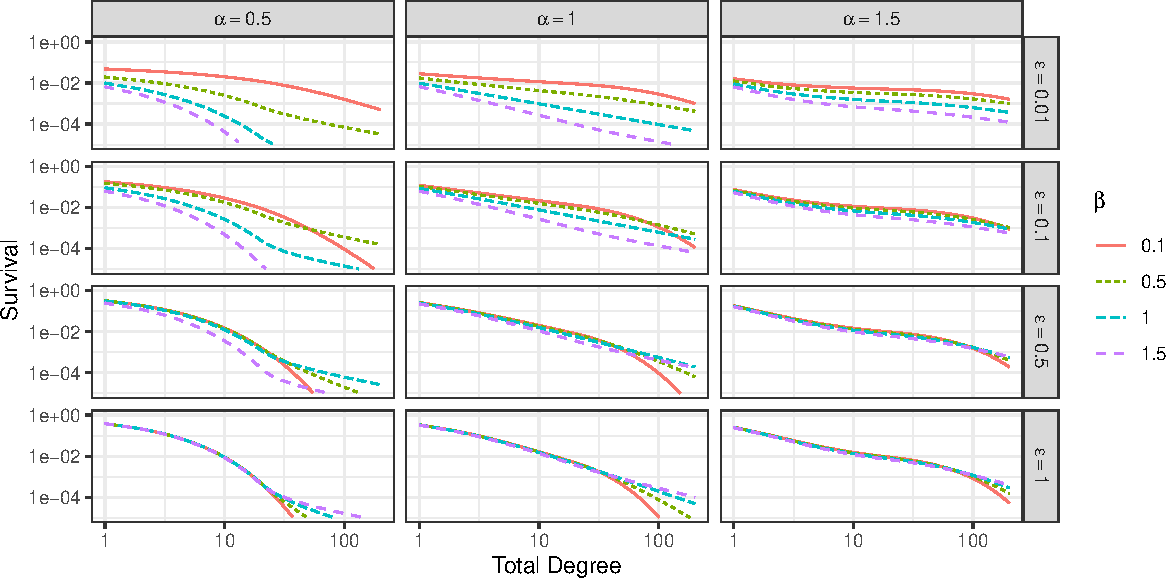
\includegraphics[width=119mm,height=\textheight,keepaspectratio]{paper_files/figure-pdf/fig-polylinsurv-1.pdf}

}

\caption{\label{fig-polylinsurv}The limiting survival, according to
various combinations of \((\alpha, \beta, \varepsilon)\) and \(k_0=20\)
of the proposed GPA model.}

\end{figure}%

Figure~\ref{fig-polylinsurv} demonstrates that this model can capture a
range of tail behaviour, including a large range of possible tail
indices ranging from 0.035 (\(\alpha=1.5, \beta=0.1, \varepsilon=1\)) to
0.999 (\(\alpha=0.5, \beta=1.5, \varepsilon=0.01\)).

An interesting property is that the analytic form of the survival
function in (\ref{eq-polysurv}), offers a natural connection to the
discrete version of the generalised Pareto (GP) distribution, providing
a link to a well established component of discrete extremes in the
literature. Specifically, it is connected to the Integer GP (IGP)
distribution seen in \citet{Rohrbeck_2018} with conditional survival: \[
\Pr(X> x|X> v) = \left(\frac{\xi(x-v)}{\sigma} + 1\right)^{-1/\xi},\qquad  x=v+1,v+2,\ldots
\] for \(v\in\mathbb Z^+, \sigma>0,\xi\in \mathbb R\), denoted as
\(X|X>u \sim  \mathrm {IGP}(\xi, \sigma, u)\) where \(\xi\) is the shape
parameter and reciprocal of the tail index.

This connection is made explicitly below, let \(\bar F (k|k\ge k_0)\) be
the conditional limiting survival of the proposed GPA model, then:

\begin{align*}
\bar F(k|k>k_0) &= \frac{\bar F(k)}{\bar F(k_0)}\\
&= \frac{\lambda^* + k_0^\alpha + \varepsilon}{k_0^\alpha + \varepsilon}\times \frac{\Gamma((\lambda^*+k_0^\alpha + \varepsilon)/\beta)}{\Gamma\left((k_0^\alpha + \varepsilon)/\beta\right)} \frac{\Gamma\left(k-k_0 + 1 +\frac{k_0^\alpha + \varepsilon}{\beta}\right)}{\Gamma\left(k-k_0 + 1 +\frac{\lambda^* +k_0^\alpha + \varepsilon}{\beta}\right)}\\
&=\frac{\Gamma(1 + (\lambda^*+k_0^\alpha + \varepsilon)/\beta)}{\Gamma\left(1+(k_0^\alpha + \varepsilon)/\beta\right)} \frac{\Gamma\left(k-k_0 + 1 +\frac{k_0^\alpha + \varepsilon}{\beta}\right)}{\Gamma\left(k-k_0 + 1 +\frac{\lambda^* +k_0^\alpha + \varepsilon}{\beta}\right)}\\
&\approx \left(1+\frac{k_0^\alpha + \varepsilon}{\beta}\right)^{\lambda^*/\beta} \left(k-k_0+1+\frac{k_0^\alpha + \varepsilon}{\beta}\right)^{-\lambda^*/\beta}\\
&=\left(\frac{\beta(k-k_0)}{k_0^{\alpha}+\varepsilon+\beta} + 1\right)^{-\lambda^{*}/\beta}
\end{align*}

Therefore, \begin{equation}\phantomsection\label{eq-igp-est}{
\bar F(k) 
\begin{cases}
=\prod_{i=0}^{k}\frac{i^\alpha + \varepsilon}{\lambda^*+i^\alpha + \varepsilon},&k\le k_0,\\
\approx \left(\prod_{i=0}^{k_0}\frac{i^\alpha + \varepsilon}{\lambda^* + i^\alpha + \varepsilon}\right)\left(\frac{\beta(k-k_0)}{k_0^{\alpha}+\varepsilon+\beta} + 1\right)^{-\lambda^{*}/\beta},&k > k_0,
\end{cases}
}\end{equation} meaning that for \(k> k_0\) the limiting degree
distribution (for large \(k_0^\alpha\)) is approximated by the
\(\text{IGP}\left(\frac{\beta}{\lambda^*}, \frac{k_0^\alpha + \varepsilon+\beta}{\lambda^*},k_0\right)\)
distribution.

To assess how close of an approximation this is, the theoretical
conditional survival Equation~\ref{eq-polysurv} are shown in
Figure~\ref{fig-approx_surv} in colour and their IGP approximations
Equation~\ref{eq-igp-est} are shown in grey. The approximation holds up
well even for large degrees and more so when \(\alpha\) is larger.

\begin{figure}

\centering{

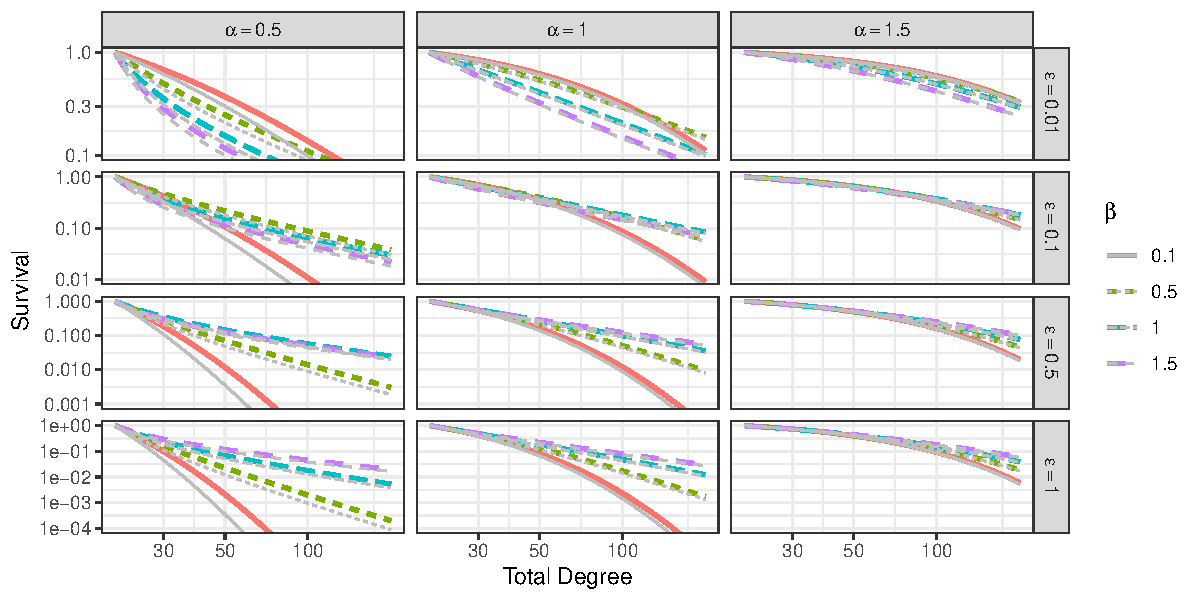
\includegraphics[width=119mm,height=\textheight,keepaspectratio]{paper_files/figure-pdf/fig-approx_surv-1.pdf}

}

\caption{\label{fig-approx_surv}Theoretical conditional survivals (grey)
of the proposed model alongside their IGP approximations (coloured).}

\end{figure}%

In agreement with Corollary~\ref{cor-omega2}, \(\beta>0\) ensures that
the shape parameter of the IGP distribution is positive and thus the
distribution is regularly varying. Additionally the shape parameter
\(\xi\) is shown in Figure~\ref{fig-polyheat} for various parameter
choices. The darker and lighter regions on the heat maps correspond to a
heavier and a lighter tail, respectively, and the red dashed line shows
combinations of \(\alpha\) and \(\beta\) that produce a limiting degree
distribution with the same tail index as the BA model.

The connection implied by Equation~\ref{eq-igp-est} is interesting
because it shows that fitting the proposed GPA model is almost
equivalent to fitting the IGP distribution to the degrees and estimating
its parameters, something that has already been done by \citet{Lee24}
with promising results. However, instead of only describing the shape of
the degree distribution, we would learn about the shape of the
preference function, thus gaining a direct understanding of the
mechanisms underlying the growth of the network.

\begin{figure}

\centering{

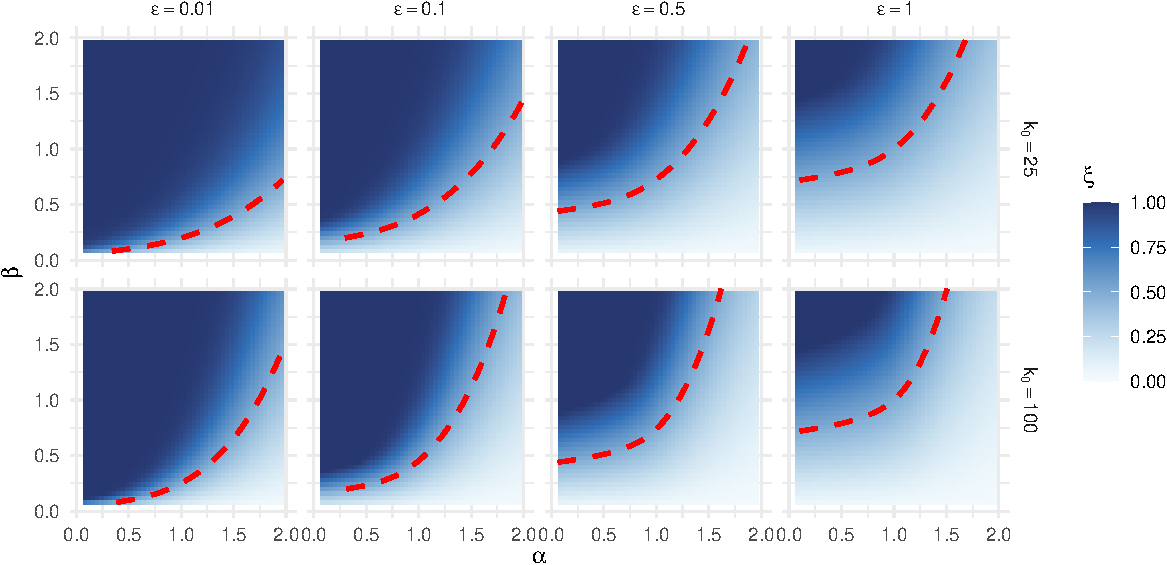
\includegraphics[width=119mm,height=\textheight,keepaspectratio]{paper_files/figure-pdf/fig-polyheat-1.pdf}

}

\caption{\label{fig-polyheat}Heat maps of \(\xi\) for various
combinations of the parameters of the proposed model.}

\end{figure}%

\newpage

To learn about the growth mechanisms, we estimate the parameters of the
proposed preference function. In order to do this we first define the
likelihood. Consider a network with degree count vector
\(\pmb n = (n_0, n_1, \ldots, n_M)\), where \(M\) is the maximum degree
and \(n_i\) being the number of nodes in the network with degree \(i\).
Using Equation~\ref{eq-pmf-origin}, the likelihood is:

\begin{equation}\phantomsection\label{eq-llh}{
\begin{aligned}
L(\pmb n | \pmb \theta,l) = &\left(\frac{\lambda^*}{\lambda^*+\varepsilon}\right)^{n_0}\left(\prod_{j=l}^{k_0-1}\frac{j^\alpha +\varepsilon}{\lambda^* + j^\alpha +\varepsilon}\right)^{\left(\sum_{i\ge k_0}n_{i}\right)} \\ &\times \prod_{l \le i<k_0}\left(\frac{\lambda^*}{\lambda^* +i^\alpha + \varepsilon } \prod_{j=l}^{k_0-1}\frac{j^\alpha + \varepsilon}{\lambda^* + j^\alpha + \varepsilon}\right)^{n_i}\\ &\times \prod_{i\ge k_0}\left(\frac{\text{B}(i-k_0 + (k_0^\alpha + \varepsilon)/\beta,1+\lambda^*/\beta)}{\text{B}((k_0^\alpha + \varepsilon)/\beta,\lambda^*/\beta)}\right)^{n_i},
\end{aligned}
}\end{equation} where \(\text{B}(\cdot,\cdot)\) is the the beta
function, \(\pmb \theta = (\alpha, \varepsilon, k_0,\beta)\), and
\(l\ge0\) is a quantity that allows truncating the data such that the
minimum degree is \(l\). This will allow the model to be fitted whilst
ignoring the influence of the lower degrees (those less than \(l\)) as
the model does not capture the behaviour well at the lower degrees,
since \citet{rudas07} only provides results for the case of a
preferential attachment tree.

The methodology for the Bayesian inference of the parameters is detailed
in Section~\ref{sec-sim}.

\section{Applications}\label{applications}

\subsection{Simulated Data}\label{sec-sim}

This subsection aims to show that the parameters of the proposed model
(and therefore the preference function) in Section~\ref{sec-model} can
be recovered from simulating a network from the model, and fitting it to
the observed degree distribution, using the likelihood in
Equation~\ref{eq-llh}.

The procedure for recovering the parameters begins with simulating a
network from the model with \(N=100,000\) vertices and \(m=1\) given
some set of parameters
\(\pmb\theta = (\alpha, \beta, \varepsilon, k_0)\). In order to carry
out the Bayesian inference of the parameters we must first assign
priors, for the parameters defined on the positive real line
(\(\alpha, \beta,\varepsilon\)) we use diffuse gamma priors and for
\(k_0\) we use a discrete uniform prior over a large and reasonable
range of values, specifically we use the priors below:

\begin{align*}
\alpha&\sim \text{Gamma}(1,0.01),\\
\beta &\sim  \text{Gamma}(1,0.01),\\
k_0 &\sim \text{U}(1,10,000),\\
\varepsilon &\sim \text{Gamma(1,0.01)},
\end{align*}

where Gamma(\(a\), \(b\)) is the gamma distribution with shape \(a\) and
rate \(b\), and U(\(a\), \(b\)) is discrete uniform distribution with
lower and upper bounds \(a\) and \(b\), to obtain a posterior
distribution, up to the proportionality constant. Posterior samples can
then be obtained by an adaptive Metropolis-Hastings Markov chain Monte
Carlo (MCMC) algorithm. For these simulated networks \(l=0\).

\begin{figure}

\centering{

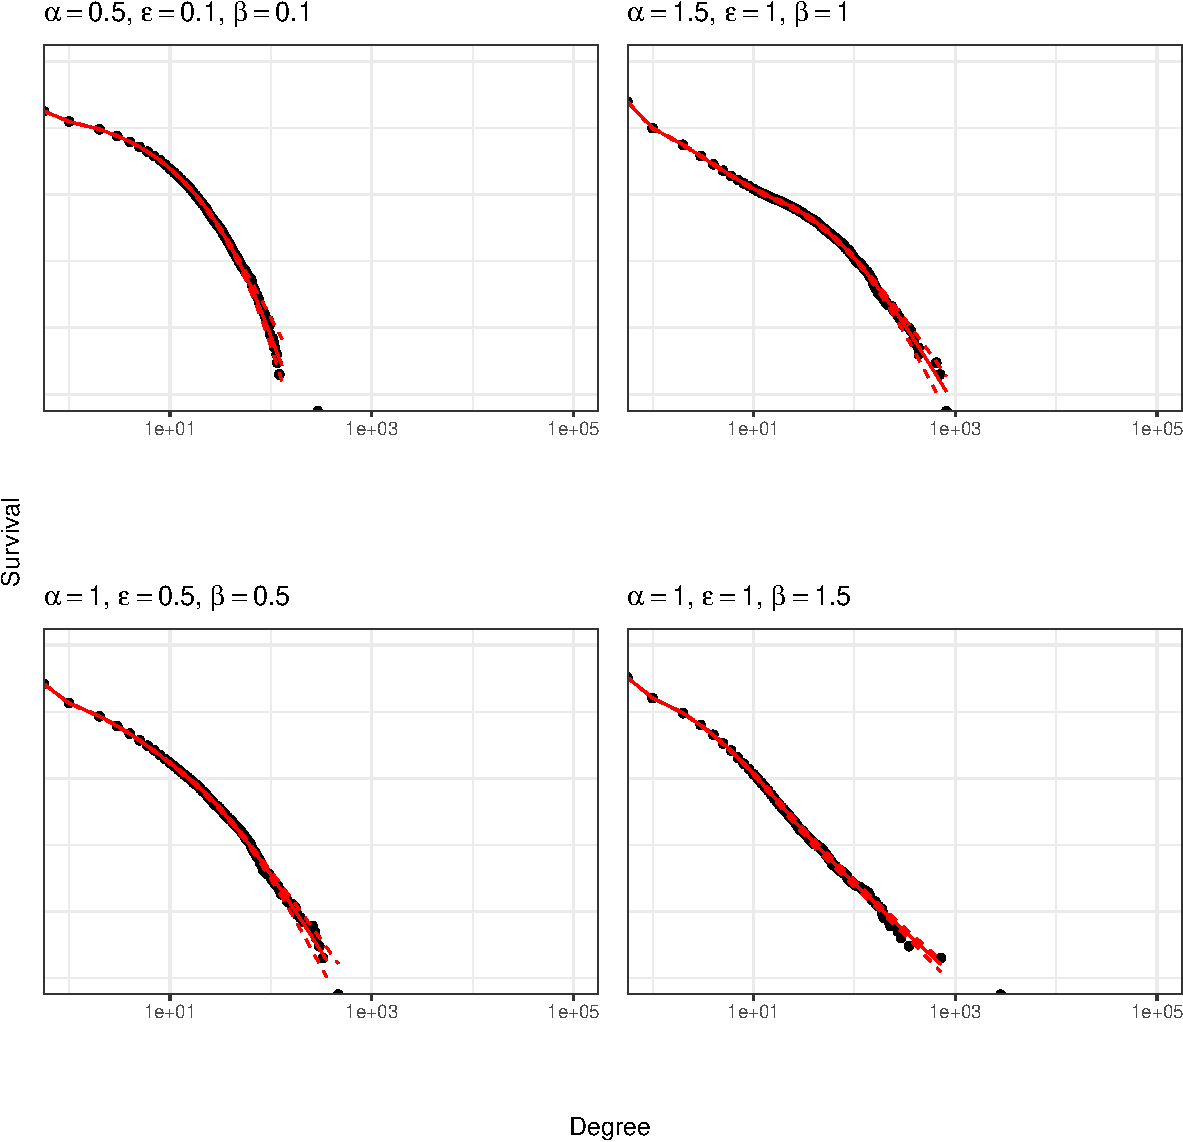
\includegraphics[width=119mm,height=\textheight,keepaspectratio]{paper_files/figure-pdf/fig-rec1-1.pdf}

}

\caption{\label{fig-rec1}Empirical (black dots) and fitted (red line)
survival functions for data simulated from the proposed model with
various combinations of \((\alpha,\beta,\epsilon)\) and \(k_0=20\). The
95\% credible (dashed lines) are included but too narrow to be seen
clearly.}

\end{figure}%

\begin{figure}

\centering{

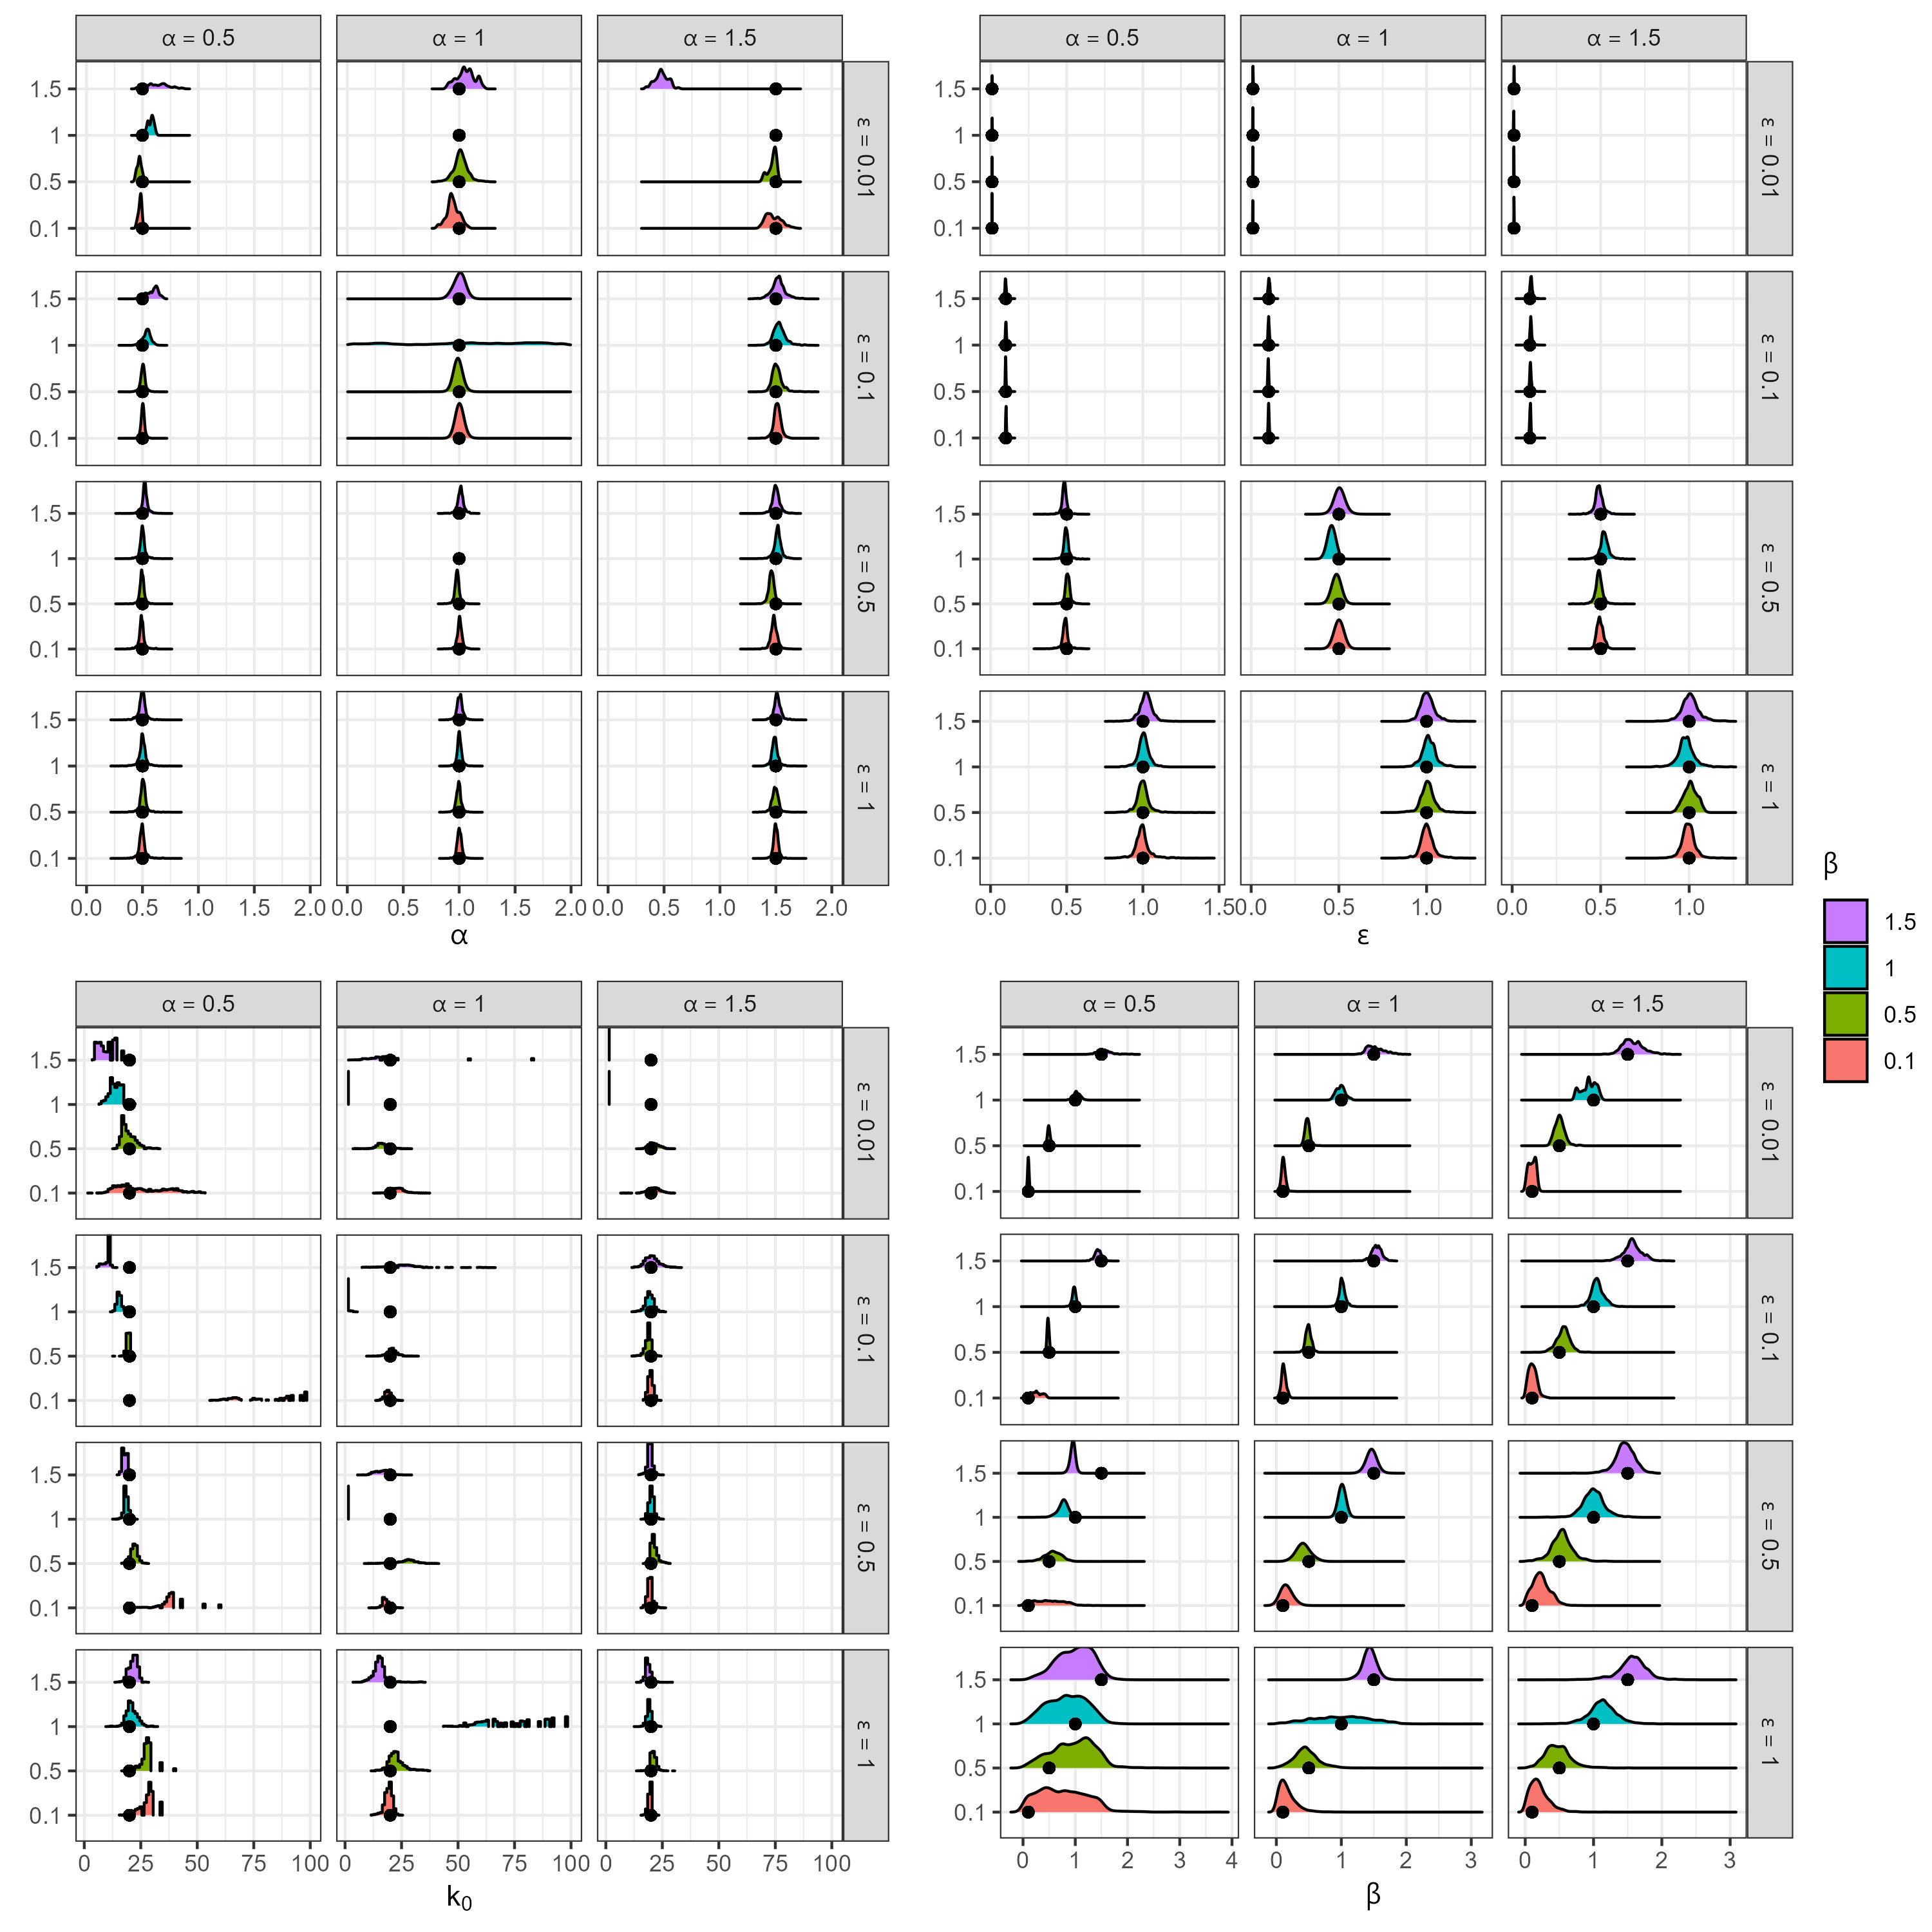
\includegraphics[width=1\linewidth,height=\textheight,keepaspectratio]{images/mcmc_plot.jpg}

}

\caption{\label{fig-rec2}: Posterior densities of parameters for data
simulated from the proposed model with various combinations of
(\(\alpha\),\(\beta\),\(\varepsilon\)) and \(k_0=20\). True parameter
values shown with black dots.}

\end{figure}%

Figures \ref{fig-rec1} and \ref{fig-rec2} demonstrate the usefulness of
the model, as we can recover the model parameters well from only the
final degree distribution of the simulated network. This indicates that
the method may also be applied to real networks, with the assumption
that they evolved according to the proposed GPA scheme.

\subsection{Real Data}\label{sec-real}

In this subsection, we fit the proposed model to the degree
distributions of various real networks and learn about the mechanics of
their growth. While we also compare the fit to that of the mixture
distribution by \citet{Lee24} we note that the proposed method has the
additional benefit of learning directly about the growth of a network
from the inference results. The data consists of 12 networks sourced
from \href{konect.cc}{KONECT} and the
\href{https://networkrepository.com}{Network Data Repository}\citep{nr}:

\begin{itemize}
\tightlist
\item
  \texttt{as-caida20071105}: network of autonomous systems of the
  Internet connected with each other from the CAIDA project
\item
  \texttt{dimacs10-astro-ph} : co-authorship network from the
  ``astrophysics'' section (astro-ph) of arXiv
\item
  \texttt{ego-twitter}: network of twitter followers
\item
  \texttt{facebook-wosn-wall}: subset of network of Facebook wall posts
\item
  \texttt{maayan-faa}: USA FAA (Federal Aviation Administration)
  preferred routes as recommended by the NFDC (National Flight Data
  Center)
\item
  \texttt{maayan-Stelzl}: network representing interacting pairs of
  proteins in humans
\item
  \texttt{moreno-blogs-blogs}: network of URLs found on the first pages
  of individual blogs
\item
  \texttt{opsahl-openflights}: network containing flights between
  airports of the world.
\item
  \texttt{pajek-erdos}:
  \(\text{co-authorship network around Paul Erd\H{o}s}\)
\item
  \texttt{reactome}: network of protein--protein interactions in humans
\item
  \texttt{sx-mathoverflow}: interactions from the StackExchange site
  \href{https://mathoverflow.net/}{MathOverflow}
\item
  \texttt{topology}: network of connections between autonomous systems
  of the Internet
\end{itemize}

The parameter inferences that follow were obtained using the same priors
and MCMC sampling method as detailed in Section~\ref{sec-sim}.

\begin{figure}

\centering{

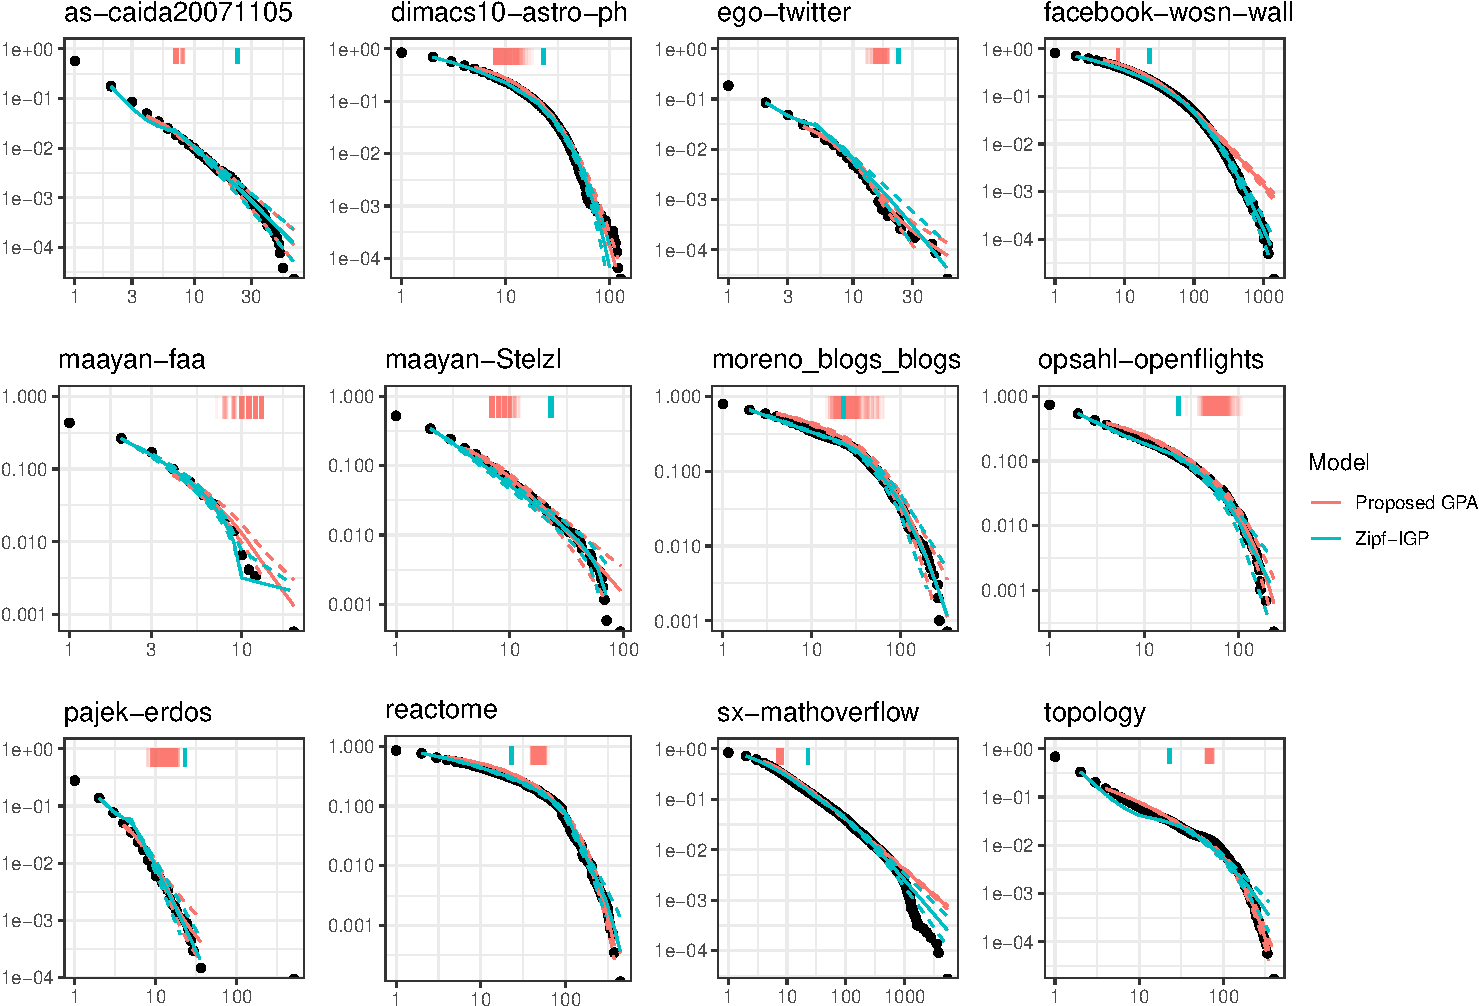
\includegraphics[width=119mm,height=\textheight,keepaspectratio]{paper_files/figure-pdf/fig-real1-1.pdf}

}

\caption{\label{fig-real1}Empirical (black dots) and posterior medians
of the fitted survival function of the proposed GPA model (solid red)
for several real data sets and their 95\% credible intervals (dotted
red). Also shown are the posterior medians (solid blue) and 95\%
credible intervals (dotted blue) for a model from \citet{Lee24}. The
corresponding \(k_0\) values are shown with short vertical lines towards
the top of each plot.}

\end{figure}%

Figure~\ref{fig-real1} displays the posterior estimates of the survival
function for various data sets, obtained from fitting the proposed GPA
model and the Zipf-IGP mixture model from \citet{Lee24}. In most cases,
the proposed GPA model gives a similar fit to the Zipf-IGP model but
where the proposed GPA model fits well we gain additional information
about the preference function, assuming that the network evolved
according the the proposed GPA scheme.

Figure~\ref{fig-shapes} shows the posterior of the shape parameter
\(\xi\) obtained from the Zipf-IGP model alongside the posterior of the
equivalent shape parameter \(\beta/\lambda^*\) obtained from fitting the
proposed GPA model. Generally, the proposed GPA model performs similarly
to the Zipf-IGP when estimating the tail behaviour of the degree
distribution. In the cases of substantial discrepancies, it is either
because the proposed GPA model fits the tail better than the Zipf-IGP
model does, or because of the threshold being too low, forcing almost
all of the data to be modelled by the linear part of the GPA. This again
shows the effects that small degrees have on this model.

\begin{figure}

\centering{

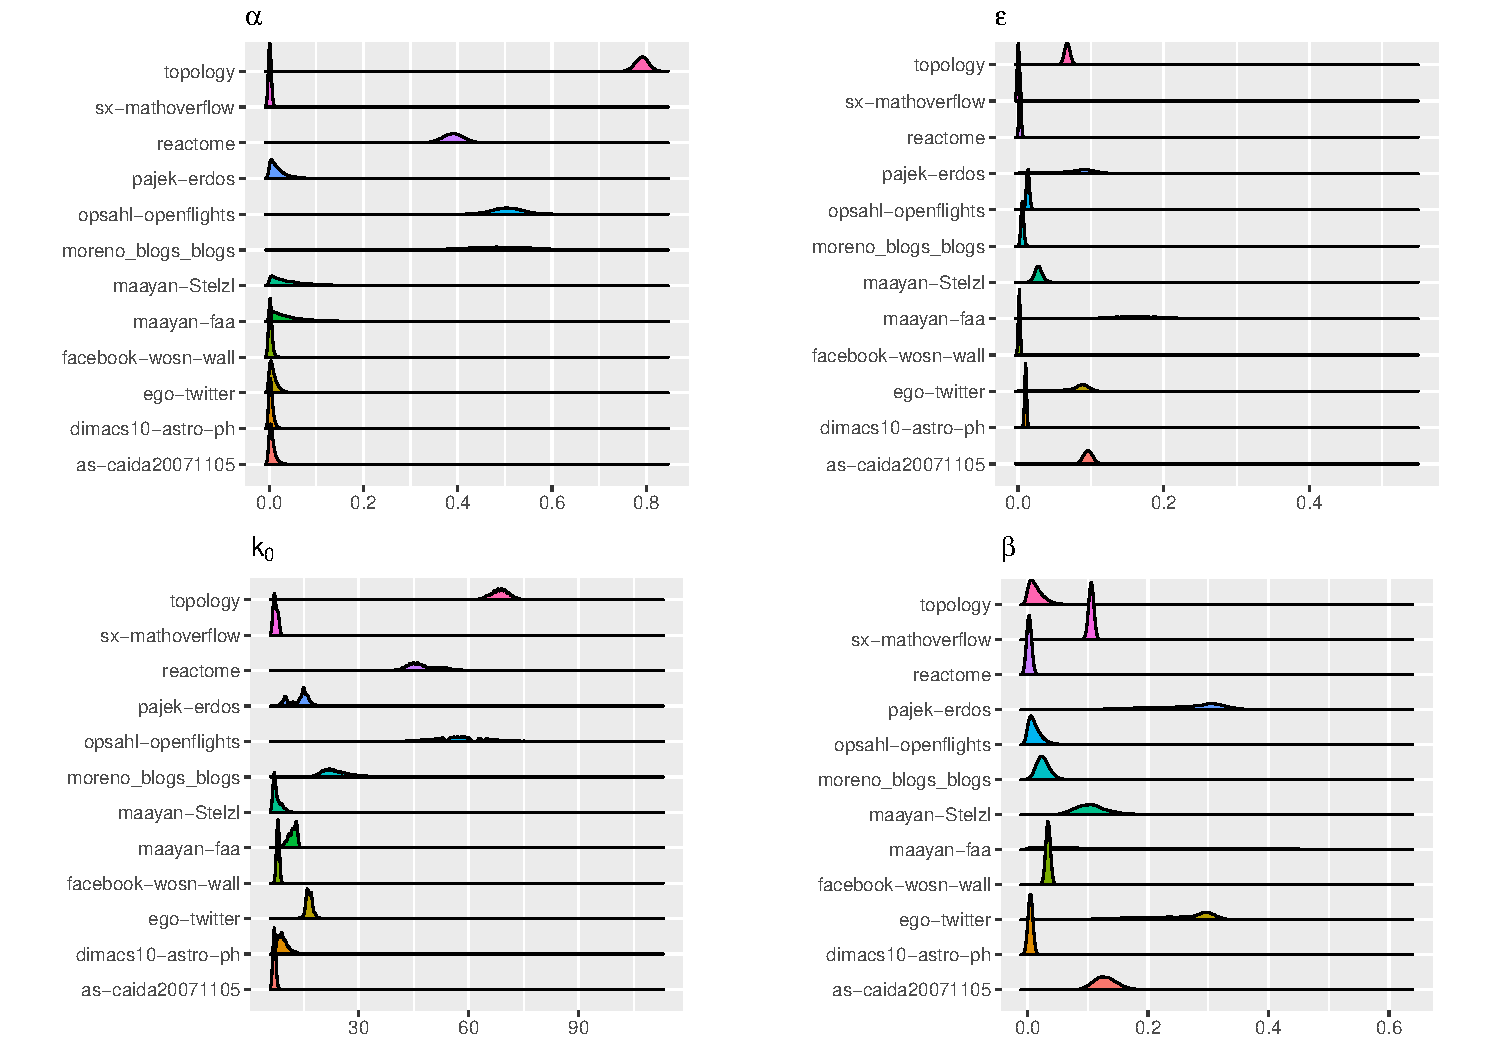
\includegraphics[width=119mm,height=\textheight,keepaspectratio]{paper_files/figure-pdf/fig-parplot-1.pdf}

}

\caption{\label{fig-parplot}Posterior densities of the parameters of the
proposed model fitted to real data.}

\end{figure}%

\begin{figure}[H]

\centering{

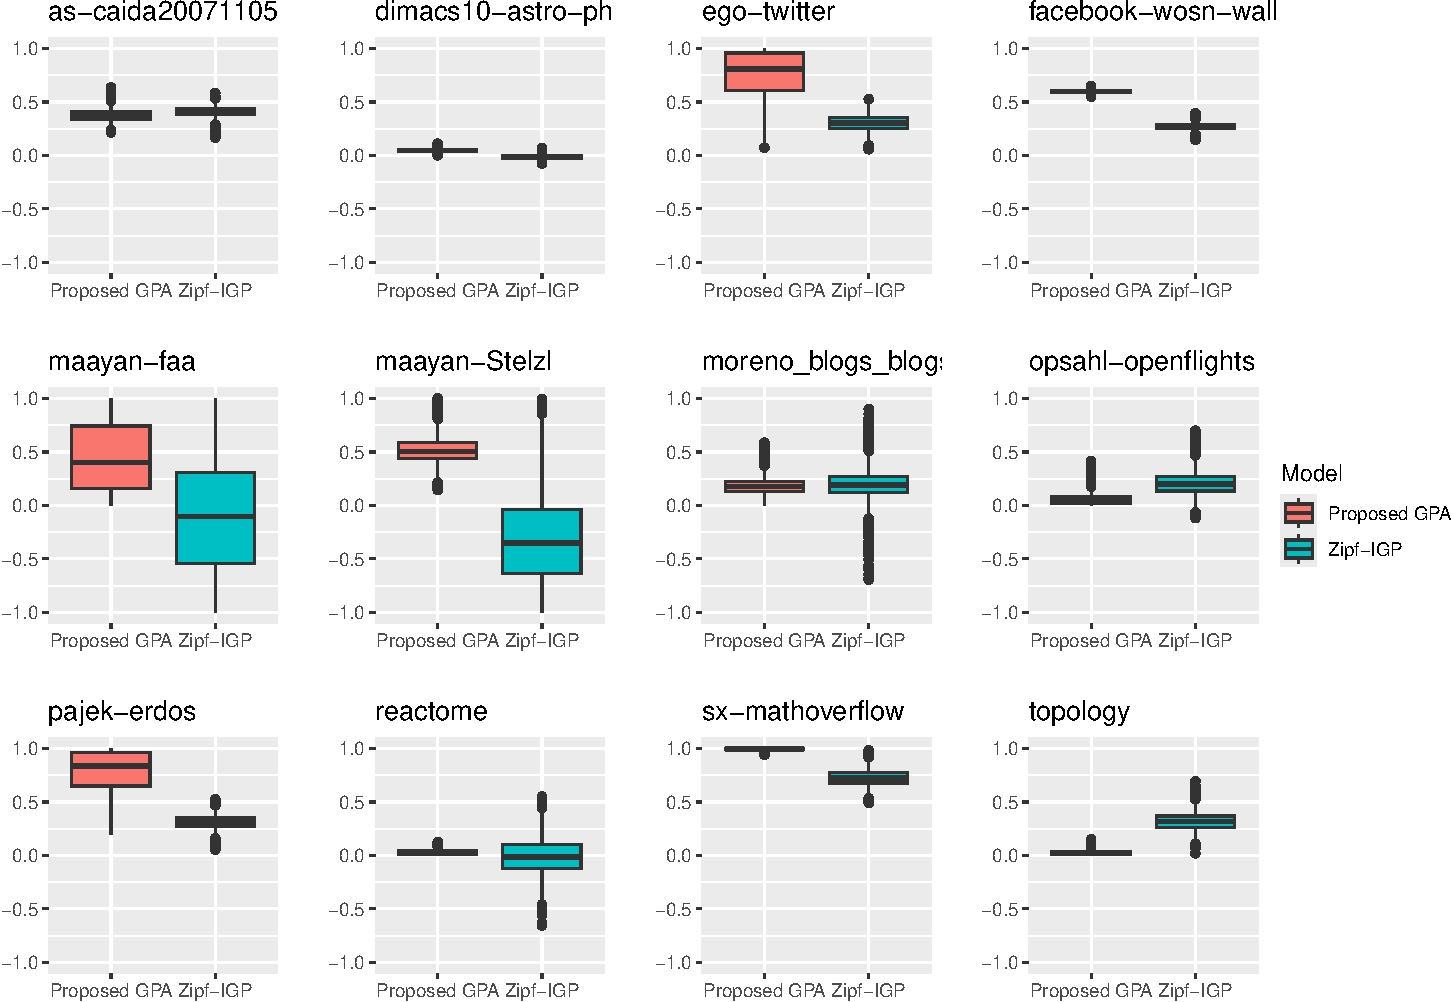
\includegraphics[width=119mm,height=\textheight,keepaspectratio]{paper_files/figure-pdf/fig-shapes-1.pdf}

}

\caption{\label{fig-shapes}Posterior estimates of shape parameter of
Zipf-IGP distribution (right) and the analagous quantity obtained from
fitting the proposed model (left).}

\end{figure}%

Figure~\ref{fig-pa} shows the estimated preference function \(b(k)\)
alongside the 95\% credible interval on a log-log scale. Although the
credible interval becomes very large for the largest degrees, this is
expected as not all of these networks had data in that region, and for
those that do the credible interval is much narrower, as is the case for
\texttt{sx-mathoverflow}. Looking at the shape of the preference
function, there appears to be two distinct shapes of preference
function. The first appears mostly flat (similar to uniform attachment)
for the smallest degrees and then after a threshold PA kicks in, some
with this shape are \texttt{pajek-erdos} and \texttt{sx-mathoverflow}.
The second distinct shape appears to provide some clear PA behaviour
that then slows down after a certain point, and examples of this are
seen in the two infrastructure networks \texttt{opsahl-openflights} and
\texttt{topology}. This slowing down could be viewed as a kind of
diminishing returns on the degree of a vertex i.e.~as a vertex gets
larger gaining more connections has less of an effect than it did before
some threshold \(k_0\).

\begin{figure}[H]

\centering{

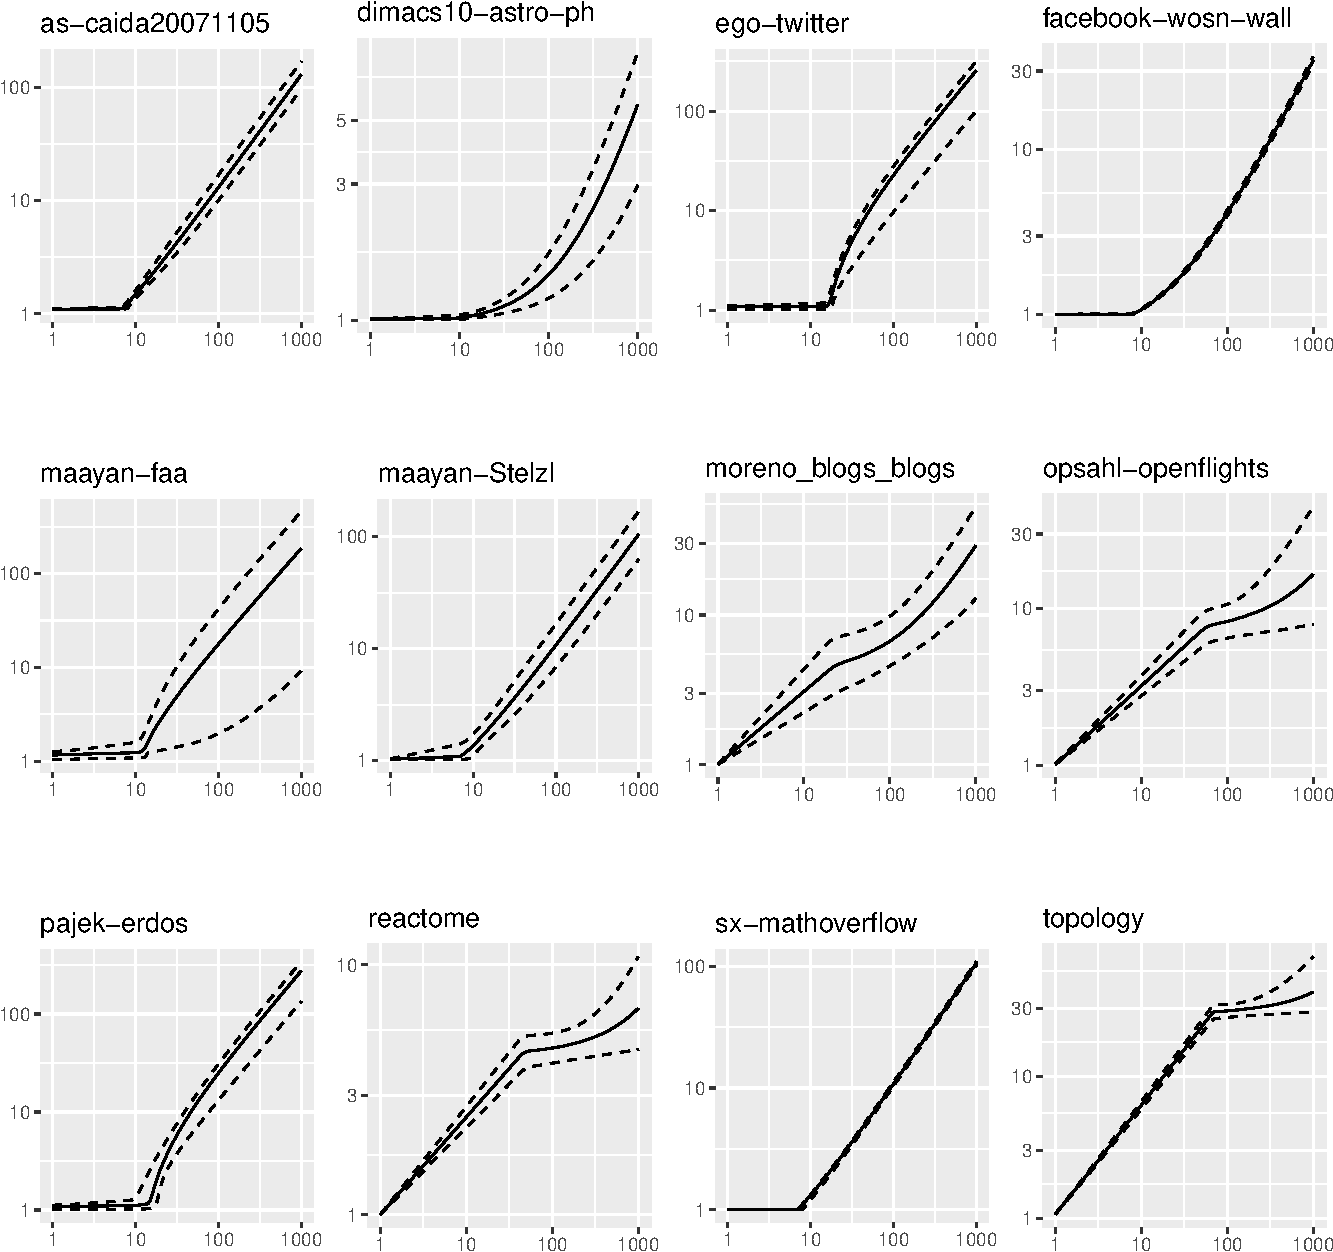
\includegraphics[width=119mm,height=\textheight,keepaspectratio]{paper_files/figure-pdf/fig-pa-1.pdf}

}

\caption{\label{fig-pa}Posterior median for the preference function
(solid) with 95\% credible interval (dashed) on log-log scale.}

\end{figure}%

\newpage

\section{Conclusion and Discussion}\label{sec-conc}

We introduced a class of preference functions that, under the GPA
scheme, generate a network with a flexible yet regularly varying degree
distribution. From the simulation study we showed that the parameters
can be recovered from fitting the model to the degrees alone. We also
applied this method to the degree distributions of real networks,
estimating their model parameters assuming they evolved in the same way.
Not only did this yield good fits for the degree distribution, similar
to that of the Zipf-IGP, it also came with the added benefit of giving a
posterior estimate for a preference function.

This paper contributes to the understanding of the relationship between
the mechanism underlying a networks growth and the resulting degree
distribution. As well as demonstrating that under certain conditions
information about this mechanism can be garnered from the degrees alone.
In future, something similar could be done by looking at another
statistic for the network (e.g.~the triangle distribution) and using it
in combination with the degrees to gain further insights into the growth
mechanism when the networks full evolution is not available. The
triangle distribution would be a good avenue for future work within the
realm of extremes as it has also been shown by \citet{kang11} that many
real networks seem to have power law triangle distributions.

One limitation of this method is that the lowest degrees needed to be
truncated as they had a very large effect on the fit of the model, as a
result of using theory developed for trees and applying it to general
networks. Future work could apply theory developed for general networks
using a similar method to this, allowing us to compare the results here
something that is more accurate. This could include fixing the
out-degree of new nodes at a constant greater than one, or allowing the
out-degree of new nodes to vary.

Its worth noting the recent work by \citet{banerjee25}, that provides
results for more general networks beyond trees utilising the same
underlying branching process. They consider a model that grows in the
exact same way as the model that we have considered, but then they
collapse the nodes of the tree resulting in a more general network much
more like those in reality. However, there is no expression for the
probability mass function of the degrees and therefore no likelihood
that can be used for modeling in the same way that we have. In spite of
this, using Remark 2 from \citet{banerjee25} it can be shown that the
survival function of the limiting degree distribution (when using a
preference function of the form from Corollary~\ref{cor-omega2}) can be
bounded by two regularly varying functions showing that the degree
distribution is still heavy tailed, although not necessarily regularly
varying.

Obtaining an expression for the degree distributions of more general
cases of preferential attachment models are, for the moment, seemingly
inaccessible and provide a real barrier to using more realistic models
in a way similar to what we have in this paper, we leave these open
problems for future analysis.

\setcounter{section}{0}
\renewcommand{\thesection}{\Alph{section}}
\setcounter{table}{0}
\renewcommand{\thetable}{A\arabic{table}}
\setcounter{figure}{0}
\renewcommand{\thefigure}{A\arabic{figure}}

\newpage

\section{Proofs and Derivations}\label{sec-proofs}

\subsection{Preliminary}\label{preliminary}

Taking the form of the GPA degree survival from
Equation~\ref{eq-surv-origin} : \[
\bar F(k) = \prod_{i=0}^k\frac{b(i)}{\lambda^*+b(i)}
\] and substituting into the formula for \(\Omega(F,n)\):

\begin{align*}
\Omega(F,k)&=\left(\log\frac{\prod_{i=0}^{k+1}\frac{b(i)}{\lambda^{*}+b(i)}}{\prod_{i=0}^{k+2}\frac{b(i)}{\lambda^{*}+b(i)}}\right)^{-1}-\left(\log\frac{\prod_{i=0}^{k}\frac{b(i)}{\lambda^{*}+b(i)}}{\prod_{i=0}^{k+1}\frac{b(i)}{\lambda^{*}+b(i)}}\right)^{-1}\\
&=\left(\log\frac{\lambda^{*}+b(k+2)}{b(k+2)}\right)^{-1}-\left(\log\frac{\lambda^{*}+b(k+1)}{b(k+1)}\right)^{-1}\\
&=\left(\log\left[1+\frac{\lambda^{*}}{b(k+2)}\right]\right)^{-1}-\left(\log\left[1+\frac{\lambda^{*}}{b(k+1)}\right]\right)^{-1}.
\end{align*}

\subsection{\texorpdfstring{Proof of
Remark~\ref{rem-omega}}{Proof of Remark~}}\label{sec-remproof}

As it is assumed throughout that \(b(k)\) is non-decreasing, we consider
the two cases where \(b(k)\) is bounded and unbounded. When \(b(k)\) is
bounded, by the monotone convergence theorem,
\(\lim_{k\rightarrow\infty}b(k) = c\) for some \(c>0\), which implies
that
\(\lim_{k\rightarrow\infty}\Omega(F,k)=\left(\log\left[1+\frac{\lambda^{*}}{c}\right]\right)^{-1}-\left(\log\left[1+\frac{\lambda^{*}}{c}\right]\right)^{-1}= 0\).
This proves the first part of Remark~\ref{rem-omega}. Now, using
Equation~\ref{eq-surv-origin},
\(\frac{\bar{F}(k+1)}{\bar{F}(k)}=\frac{b(k+1)}{\lambda^{*}+b(k+1)}\rightarrow\frac{c}{\lambda^{*}+c}<1\)
as \(k\rightarrow\infty\). This means that \(F\) is not long-tailed, and
therefore is only recovered to the Gumbel MDA.

\subsection{\texorpdfstring{Proof of
Proposition~\ref{prp-omega}}{Proof of Proposition~}}\label{sec-prpproof}

Now we consider the case where \(b(k)\) is unbounded, re-write
\(\Omega(F,k)\) as:

\begin{align*}
\Omega(F,k) &= \left(\log\left[1+\frac{\lambda^{*}}{b(k+2)}\right]\right)^{-1}-\frac{b(k+2)}{\lambda^{*}}+\frac{b(k+2)}{\lambda^{*}}\\&\qquad  -\left(\log\left[1+\frac{\lambda^{*}}{b(k+1)}\right]\right)^{-1}+\frac{b(k+1)}{\lambda^{*}}-\frac{b(k+1)}{\lambda^{*}}\\
&=\left\{ \left(\log\left[1+\frac{\lambda^{*}}{b(k+2)}\right]\right)^{-1}-\frac{b(k+2)}{\lambda^{*}}\right\}\\ &\qquad  - \left\{ \left(\log\left[1+\frac{\lambda^{*}}{b(k+1)}\right]\right)^{-1}-\frac{b(k+1)}{\lambda^{*}}\right\}\\&\qquad  +\frac{b(k+2)}{\lambda^{*}}-\frac{b(k+1)}{\lambda^{*}}.
\end{align*}

Then as \(\lim_{k\rightarrow\infty}b(k)=\infty\) it follows that:

\begin{align*}
\lim_{k\rightarrow\infty}\Omega(F,k) &= \lim_{k\rightarrow\infty}\left\{ \left(\log\left[1+\frac{\lambda^{*}}{b(k+2)}\right]\right)^{-1}-\frac{b(k+2)}{\lambda^{*}}\right\} \\&\qquad - \lim_{k\rightarrow\infty}\left\{ \left(\log\left[1+\frac{\lambda^{*}}{b(k+1)}\right]\right)^{-1}-\frac{b(k+1)}{\lambda^{*}}\right\}\\
&\qquad +\lim_{k\rightarrow\infty}\left(\frac{b(k+2)}{\lambda^{*}}-\frac{b(k+1)}{\lambda^{*}}\right)\\
&=\frac{1}{2}-\frac{1}{2} + \lim_{k\rightarrow\infty}\left(\frac{b(k+2)}{\lambda^{*}}-\frac{b(k+1)}{\lambda^{*}}\right)\\
&=\frac{1}{\lambda^{*}}\lim_{k\rightarrow\infty}\left[b(k+2)-b(k+1)\right].\qquad  \square
\end{align*}

The first two lines both have the limit \(1/2\) as
\(\lim_{z\rightarrow{}0}\left[\log(1+z)\right]^{-1}-z^{-1} = 1/2\).

Now, using Equation~\ref{eq-surv-origin},
\(\frac{\bar{F}(k+1)}{\bar{F}(k)}=\frac{b(k+1)}{\lambda^{*}+b(k+1)}=\frac{1}{\lambda^{*}/b(k+1) + 1}\rightarrow{}1\)
as \(k\rightarrow\infty\). This means that \(F\) is long-tailed, and
therefore is in an MDA.

\subsection{\texorpdfstring{Derivation of
Equation~\ref{eq-rho}}{Derivation of Equation~}}\label{sec-rhoproof}

For a preference function of the form:

\[
b(k) = \begin{cases}
g(k),&k\le k_0,\\
g(k_0) + \beta(k-k_0), &k> k_0,
\end{cases}
\] for \(\beta>0, k_0\in\mathbb N\) we have that

\begin{align*}
\hat\rho(\lambda) &= \sum_{n=0}^\infty\prod_{i=0}^{n-1}\frac{b(i)}{\lambda+b(i)}\\ &= \sum_{n=0}^{k_0}\prod_{i=0}^{n-1}\frac{g(i)}{\lambda+g(i)} + \sum_{n=k_0+1}^\infty\left(\prod_{i=0}^{k_0-1}\frac{g(i)}{\lambda+g(i)}\prod_{i=k_0}^{n-1}\frac{g(k_0) + \beta(i-k_0)}{\lambda +g(k_0) + \beta(i-k_0)}\right)\\
&=\sum_{n=0}^{k_0}\prod_{i=0}^{n-1}\frac{g(i)}{\lambda+g(i)} + \left(\prod_{i=0}^{k_0-1}\frac{g(i)}{\lambda+g(i)}\right)\sum_{n=k_0+1}^\infty\prod_{i=k_0}^{n-1}\frac{g(k_0) + \beta(i-k_0)}{\lambda +g(k_0) + \beta(i-k_0)}.
\end{align*}

Now using the fact that:

\[
\prod_{i=0}^n(x+yi) = x^{n+1}\frac{\Gamma\left(\frac{x}{y}+n+1\right)}{\Gamma\left(\frac{x}{y}\right)}
\] and reindexing the product in the second sum,

\begin{align*}
\hat\rho(\lambda) &= C_{g,k_0} + \left(\prod_{i=0}^{k_0-1}\frac{g(i)}{\lambda+g(i)}\right)\sum_{n=k_0+1}^\infty\frac{\Gamma\left(\frac{g(k_0)}{\beta}+n-k_0\right)\Gamma\left(\frac{\lambda+g(k_0)}{\beta}\right)}{\Gamma\left(\frac{\lambda+g(k_0)}{\beta}+n-k_0\right)\Gamma\left(\frac{g(k_0)}{\beta}\right)}\\
&= C_{g,k_0} + \frac{\Gamma\left(\frac{\lambda+g(k_0)}{\beta}\right)}{\Gamma\left(\frac{g(k_0)}{\beta}\right)}\left(\prod_{i=0}^{k_0-1}\frac{g(i)}{\lambda+g(i)}\right)\sum_{n=k_0+1}^\infty\frac{\Gamma\left(\frac{g(k_0)}{\beta}+n-k_0\right)}{\Gamma\left(\frac{\lambda+g(k_0)}{\beta}+n-k_0\right)}\\
&=C_{g,k_0} + \frac{\Gamma\left(\frac{\lambda+g(k_0)}{\beta}\right)}{\Gamma\left(\frac{g(k_0)}{\beta}\right)}\left(\prod_{i=0}^{k_0-1}\frac{g(i)}{\lambda+g(i)}\right)\sum_{n=1}^\infty\frac{\Gamma\left(\frac{g(k_0)}{\beta}+n\right)}{\Gamma\left(\frac{\lambda+g(k_0)}{\beta}+n\right)},
\end{align*}

where
\(C_{g,k_0} = \sum_{n=0}^{k_0}\prod_{i=0}^{n-1}\frac{g(i)}{\lambda+g(i)}\).

In order to simplify the infinite sum, consider:

\begin{align*}
\sum_{n=0}^\infty\frac{\Gamma(n+x)}{\Gamma(n+x+y)} &=\frac{1}{\Gamma(y)}\sum_{n=0}^\infty \text{B}(n+x,y)\\
&=\frac{1}{\Gamma(y)}\sum_{n=0}^\infty\int_0^1t^{n+x-1}(1-t)^{y-1}\text{d}t\\
&=\frac{1}{\Gamma(y)}\int_0^1 t^{x-1}(1-t)^{y-1}\sum_{n=0}^\infty t^n \text{d}t\\
&=\frac{1}{\Gamma(y)}\int_0^1 t^{x-1}(1-t)^{y-1}\frac{1}{1-t}\text{d}t\\
&=\frac{1}{\Gamma(y)}\int_0^1 t^{x-1}(1-t)^{y-2}\text{d}t\\
&=\frac{1}{\Gamma(y)}\text{B}(x,y-1)\\
&= \frac{\Gamma(x)}{(y-1)\Gamma(x+y-1)}.
\end{align*}

This infinite sum does not converge when \(x\le1\) as each term is
\(O(n^{-x})\). We can now use this in \(\hat\rho(\lambda)\):

\begin{align*}
\hat\rho(\lambda) &= C_{g,k_0} + \frac{\Gamma\left(\frac{\lambda+g(k_0)}{\beta}\right)}{\Gamma\left(\frac{g(k_0)}{\beta}\right)}\left(\prod_{i=0}^{k_0-1}\frac{g(i)}{\lambda+g(i)}\right)\\&\qquad \times\left(\frac{\Gamma\left(\frac{g(k_0)}{\beta}\right)}{\left(\frac{\lambda}{\beta}-1\right)\Gamma\left(\frac{g(k_0)+\lambda}{\beta}-1\right)}-\frac{\Gamma\left(\frac{g(k_0)}{\beta}\right)}{\Gamma\left(\frac{g(k_0)+\lambda}{\beta}\right)}\right)\\
&=C_{g,k_0} + \left(\prod_{i=0}^{k_0-1}\frac{g(i)}{\lambda+g(i)}\right)\left(\frac{\Gamma\left(\frac{g(k_0)+\lambda}{\beta}\right)}{\left(\frac{\lambda}{\beta}-1\right)\Gamma\left(\frac{g(k_0)+\lambda}{\beta}-1\right)}-1\right)\\
&=C_{g,k_0} + \left(\prod_{i=0}^{k_0-1}\frac{g(i)}{\lambda+g(i)}\right)\left(\frac{\frac{g(k_0)+\lambda}{\beta}-1}{\frac{\lambda}{\beta}-1}-1\right)\\
&=C_{g,k_0} + \left(\prod_{i=0}^{k_0-1}\frac{g(i)}{\lambda+g(i)}\right)\left(\frac{g(k_0)+\lambda-\beta}{\lambda-\beta}-1\right)\\&=\sum_{n=0}^{k_0}\prod_{i=0}^{n-1}\frac{g(i)}{\lambda+g(i)} + \frac{g(k_0)}{\lambda-\beta}\prod_{i=0}^{k_0-1}\frac{g(i)}{\lambda+g(i)}.\qquad  \square
\end{align*}

\newpage

\section*{References}\label{references}
\addcontentsline{toc}{section}{References}

\renewcommand{\bibsection}{}
\bibliography{refs.bib}





\end{document}
